%!TEX TX-program = xelatex
\documentclass[8pt]{article}

\usepackage{ctex}
\usepackage{graphicx}
\usepackage{enumitem}
\usepackage{geometry}
\usepackage{amsmath}
\usepackage{amssymb}
\usepackage{amsfonts}
\usepackage{tikz}
\usetikzlibrary{positioning}
\usetikzlibrary{svg.path}
\usetikzlibrary{fit}
\usepackage{xcolor}
\usepackage{longtable}

\graphicspath{ {./images/} }

\title{4 幂函数、指数函数与对数函数}
\author{高一(6)班\ 邵亦成\ 26号}
% \date{202年}

\geometry{a4paper, scale=0.8}

\setcounter{section}{3}

\newcommand\addvmargin[1]{
  \node[fit=(current bounding box),inner ysep=#1,inner xsep=0]{};
}

\setlength{\tabcolsep}{5mm} % separator between columns
\def\arraystretch{1.25} % vertical stretch factor

\begin{document}

	\maketitle

	\section{幂函数、指数函数与对数函数}
		\subsection{幂函数}
			~\\

			\textbf{幂函数的定义}: 形如$$y=x^a (a\text{是常数}, a\in \mathbb{R})$$的函数叫\textbf{指数为$a$的幂函数}.

			\textbf{幂函数的图像}: 考虑函数$y=x^a, a\in \mathbb{Q}$, 令$a=\dfrac{q}{p}, p, q$为互质的整数, 则有以下11种图像:

			\begin{center}
				\begin{longtable}{c|ccc}
				&$p$奇$q$奇&$p$奇$q$偶&$p$偶$q$奇\\
				\hline\\
				$a>1$ & $\begin{tikzpicture}[scale=0.7, baseline=0]
				    		\draw[black, ->] (-3,  0)--( 3,  0);
				    		\draw[black, ->] ( 0, -3)--( 0,  3);
				    		\draw[black, domain=-2:2] plot(\x, \x ^ 1.6);
				    		\draw[black, dashed] (0, 1)--(1, 1)--(1, 0);
							\filldraw[black] (1, 1) circle (2pt) node[anchor=west] {$(1, 1)$};
    						\addvmargin{1mm}
				    	\end{tikzpicture}$ & $\begin{tikzpicture}[scale=0.7, baseline=0]
				    		\draw[black, ->] (-3,  0)--( 3,  0);
				    		\draw[black, ->] ( 0, -3)--( 0,  3);
				    		\draw[black, domain=-2:2] plot(\x, \x * \x);
				    		\draw[black, dashed] (0, 1)--(1, 1)--(1, 0);
							\filldraw[black] (1, 1) circle (2pt) node[anchor=west] {$(1, 1)$};
    						\addvmargin{1mm}
				    	\end{tikzpicture}$ & $\begin{tikzpicture}[scale=0.7, baseline=0]
				    		\draw[black, ->] (-3,  0)--( 3,  0);
				    		\draw[black, ->] ( 0, -3)--( 0,  3);
				    		\draw[black, domain=0:2] plot(\x, \x ^ 1.75);
				    		\draw[black, dashed] (0, 1)--(1, 1)--(1, 0);
							\filldraw[black] (1, 1) circle (2pt) node[anchor=west] {$(1, 1)$};
    						\addvmargin{1mm}
				    	\end{tikzpicture}$\\
				$a=1$ & $\begin{tikzpicture}[scale=0.7, baseline=0]
				    		\draw[black, ->] (-3,  0)--( 3,  0);
				    		\draw[black, ->] ( 0, -3)--( 0,  3);
				    		\draw[black, domain=-2:2] plot(\x, \x);
				    		\draw[black, dashed] (0, 1)--(1, 1)--(1, 0);
							\filldraw[black] (1, 1) circle (2pt) node[anchor=west] {$(1, 1)$};
    						\addvmargin{1mm}
				    	\end{tikzpicture}$\\
				$0<a<1$ & $\begin{tikzpicture}[scale=0.7, baseline=0]
				    		\draw[black, ->] (-3,  0)--( 3,  0);
				    		\draw[black, ->] ( 0, -3)--( 0,  3);
				    		\draw[black, domain=-2:-0.5] plot(\x, \x^ 0.6);
				    		\draw[black, domain=-0.5:0.5] plot(\x, \x^ 0.6);
				    		\draw[black, domain=0.5:2] plot(\x, \x^ 0.6);
				    		\draw[black, dashed] (0, 1)--(1, 1)--(1, 0);
							\filldraw[black] (1, 1) circle (2pt) node[anchor=north west] {$(1, 1)$};
    						\addvmargin{1mm}
				    	\end{tikzpicture}$ & $\begin{tikzpicture}[scale=0.7, baseline=0]
				    		\draw[black, ->] (-3,  0)--( 3,  0);
				    		\draw[black, ->] ( 0, -3)--( 0,  3);
				    		\draw[black, domain=-2:-0.5] plot(\x, {(\x*\x)^(1/3)});
				    		\draw[black, domain=-0.5:0.5] plot(\x, {(\x*\x)^(1/3)});
				    		\draw[black, domain=0.5:2] plot(\x, {(\x*\x)^(1/3)});
				    		\draw[black, dashed] (0, 1)--(1, 1)--(1, 0);
							\filldraw[black] (1, 1) circle (2pt) node[anchor=north west] {$(1, 1)$};
    						\addvmargin{1mm}
				    	\end{tikzpicture}$ & $\begin{tikzpicture}[scale=0.7, baseline=0]
				    		\draw[black, ->] (-3,  0)--( 3,  0);
				    		\draw[black, ->] ( 0, -3)--( 0,  3);
				    		\draw[black, domain=0:2] plot(\x, {(\x*\x*\x)^(1/4)});
				    		\draw[black, dashed] (0, 1)--(1, 1)--(1, 0);
							\filldraw[black] (1, 1) circle (2pt) node[anchor=north west] {$(1, 1)$};
    						\addvmargin{1mm}
				    	\end{tikzpicture}$\\
				$a=0$ & $\begin{tikzpicture}[scale=0.7, baseline=0]
				    		\draw[black, ->] (-3,  0)--( 3,  0);
				    		\draw[black, ->] ( 0, -3)--( 0,  3);
				    		\draw[black, domain=-2:2] plot(\x, 1);
							\draw[black] (0, 1) circle (3pt);
    						\addvmargin{1mm}
				    	\end{tikzpicture}$\\
				$a<0$ & $\begin{tikzpicture}[scale=0.7, baseline=0]
				    		\draw[black, ->] (-3,  0)--( 3,  0);
				    		\draw[black, ->] ( 0, -3)--( 0,  3);
				    		\draw[black, domain=-2:-0.5] plot(\x, 1 / \x);
				    		\draw[black, domain=0.5:2] plot(\x, 1 / \x);
				    		\draw[black, dashed] (0, 1)--(1, 1)--(1, 0);
							\filldraw[black] (1, 1) circle (2pt) node[anchor=south west] {$(1, 1)$};
    						\addvmargin{1mm}
				    	\end{tikzpicture}$ & $\begin{tikzpicture}[scale=0.7, baseline=0]
				    		\draw[black, ->] (-3,  0)--( 3,  0);
				    		\draw[black, ->] ( 0, -3)--( 0,  3);
				    		\draw[black, domain=-2:-0.75] plot(\x, {1/(\x*\x)});
				    		\draw[black, domain=0.75:2] plot(\x, {1/(\x*\x)});
				    		\draw[black, dashed] (0, 1)--(1, 1)--(1, 0);
							\filldraw[black] (1, 1) circle (2pt) node[anchor=south west] {$(1, 1)$};
    						\addvmargin{1mm}
				    	\end{tikzpicture}$ & $\begin{tikzpicture}[scale=0.7, baseline=0]
				    		\draw[black, ->] (-3,  0)--( 3,  0);
				    		\draw[black, ->] ( 0, -3)--( 0,  3);
				    		\draw[black, domain=0.25:2] plot(\x, {(\x)^(-1/2)});
				    		\draw[black, dashed] (0, 1)--(1, 1)--(1, 0);
							\filldraw[black] (1, 1) circle (2pt) node[anchor=south west] {$(1, 1)$};
    						\addvmargin{1mm}
				    	\end{tikzpicture}$\\
				\end{longtable}
			\end{center}

			\textbf{幂函数的定义域}: (1) $\mathbb{R}$: $a>1$且$p$奇 or $a=1$ or $0<a<1$且$p$奇; (2) $[0, +\infty)$: $a>1$且$p$偶 or $0<a<1$且$p$偶; (3) $(-\infty, 0)\cup(0, +\infty)$: $a=0$ or $a<0$且$p$奇; (4) $(0. +\infty)$: $a<0$且$p$偶.

			\textbf{幂函数的值域}: (1) $\mathbb{R}$: $a>1$且$p$奇$q$奇 or $a=1$ or $0<a<1$且$p$奇$q$奇; (2) $[0, +\infty)$: $a>1$且$q$偶 or $0<a<1$且$q$偶; (3) $\{1\}$: $a=1$; (4) $(-\infty, 0)\cup(0, +\infty)$: $a<0$且$p$奇$q$奇; (5) $(0, +\infty)$: $a<0$且$q$偶.

			\textbf{如何记忆幂函数的11种图像}: 第一象限 + 奇偶性.

			$$
			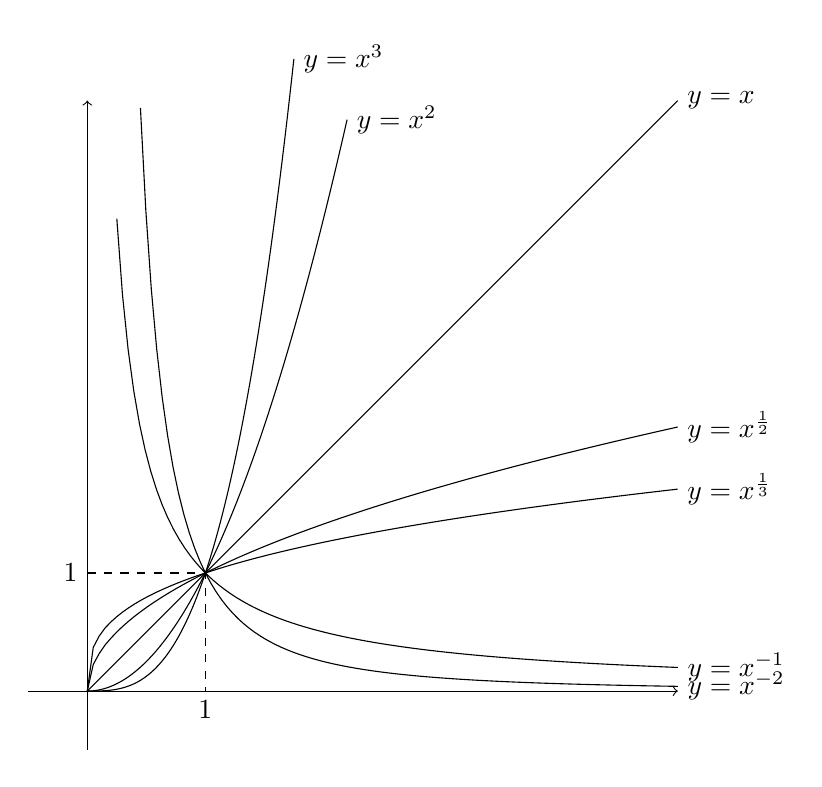
\begin{tikzpicture}[scale=1.5, baseline=0]
	    		\draw[black, ->] (-0.5,  0)--( 5,  0);
	    		\draw[black, ->] ( 0, -0.5)--( 0,  5);
	    		\draw[black, domain=0:1.75, samples=100] plot(\x, {(\x)^(3)}) node[right] {$y=x^3$};
	    		\draw[black, domain=0:2.2, samples=100] plot(\x, {(\x)^(2)}) node[right] {$y=x^2$};
	    		\draw[black, domain=0:5, samples=100] plot(\x, {(\x)^(1)}) node[right] {$y=x$};
	    		\draw[black, domain=0:5, samples=100] plot(\x, {(\x)^(1/2)}) node[right] {$y=x^{\frac{1}{2}}$};
	    		\draw[black, domain=0:5, samples=100] plot(\x, {(\x)^(1/3)}) node[right] {$y=x^{\frac{1}{3}}$};
	    		\draw[black, domain=0.25:5, samples=100] plot(\x, {(\x)^(-1)}) node[right] {$y=x^{-1}$};
	    		\draw[black, domain=0.45:5, samples=100] plot(\x, {(\x)^(-2)}) node[right] {$y=x^{-2}$};
	    		\draw[black, dashed] (0, 1)--(1, 1)--(1, 0) node at (1, 0)[anchor=north] {$1$} node at (0, 1)[anchor=east] {$1$};
				\addvmargin{1mm}
			\end{tikzpicture}
			$$

			\textbf{幂函数的通性}: (1) 在第一象限均被定义, 第四象限没有定义. (2) 过点$(1, 1)$, 且当且仅当$a>0$时过$(0,0)$. (3) $a>0$时在第一象限严格增, $a<0$时在第一象限严格减. (4) $a\leq 0$时与$x$轴, $y$轴无交点.

		\subsection{指数函数}
			~\\

			\textbf{指数函数的定义}: 形如$$y=a^x (a\text{是常数}, a>0 \text{ 且 } a\neq 1)$$的函数叫\textbf{底为$a$的指数函数}.

			\textbf{指数函数的图像}: 2种图像:

			\begin{center}
				\begin{longtable}{c|c}
					$0<a<1$&$a>1$\\
					\hline\\
					$\begin{tikzpicture}[scale=0.7, baseline=0]
			    		\draw[black, ->] (-5,  0)--( 5,  0);
			    		\draw[black, ->] ( 0, -1)--( 0,  5);
			    		\draw[black, domain=-4:4] plot(\x, {0.625 ^ \x});
			    		\filldraw[black] (0, 1) circle (0.2em) node[anchor=south west] {$1$};
						\addvmargin{1mm}
			    	\end{tikzpicture}$ & $\begin{tikzpicture}[scale=0.7, baseline=0]
			    		\draw[black, ->] (-5,  0)--( 5,  0);
			    		\draw[black, ->] ( 0, -1)--( 0,  5);
			    		\draw[black, domain=-4:4] plot(\x, {1.6 ^ \x});
			    		\filldraw[black] (0, 1) circle (0.2em) node[anchor=south east] {$1$};
						\addvmargin{1mm}
			    	\end{tikzpicture}$\\
				\end{longtable}
			\end{center}

			\textbf{如何记忆指数函数的图像}:

			$$
			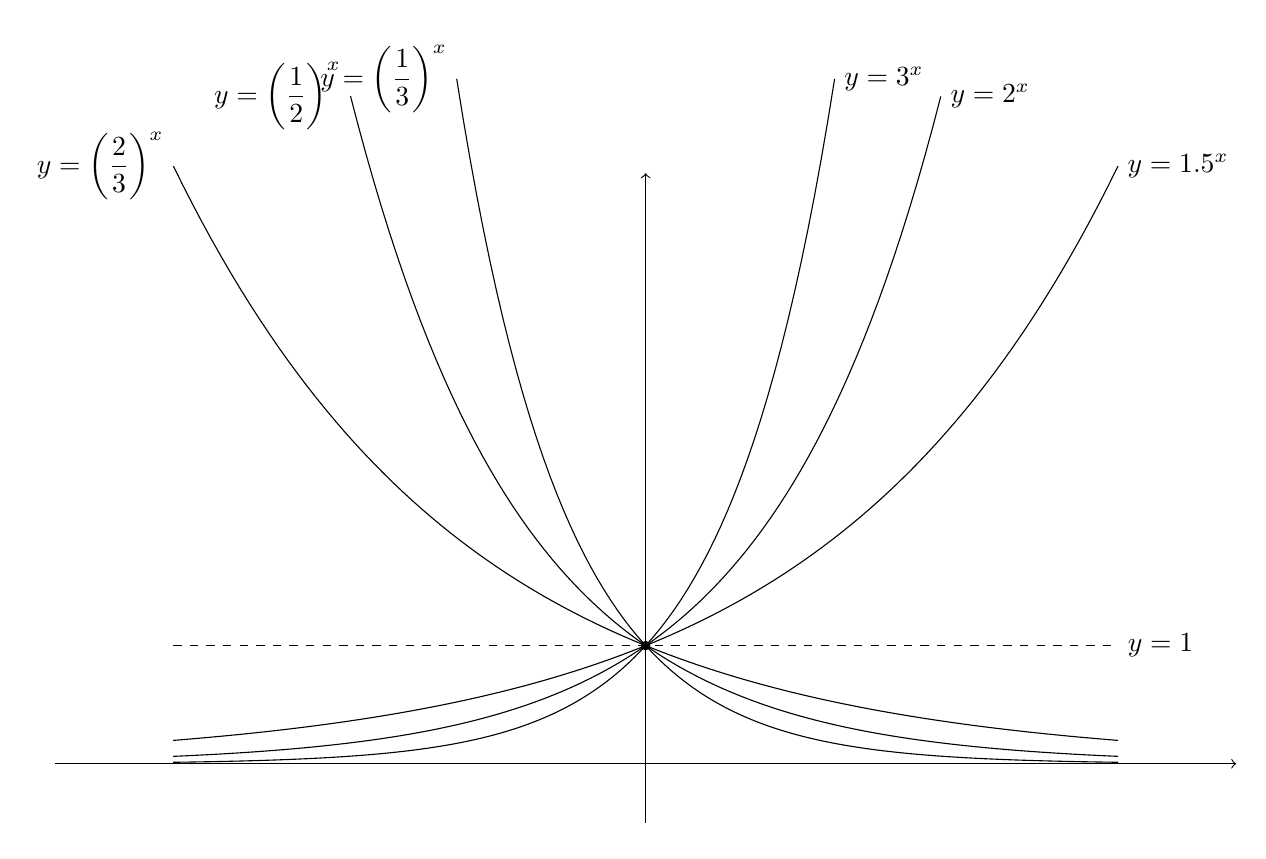
\begin{tikzpicture}[scale=1.5, baseline=0]
	    		\draw[black, ->] (-5,  0)--( 5,  0);
	    		\draw[black, ->] ( 0, -0.5)--( 0,  5);
	    		\draw[black, domain=-4:1.6, samples=100] plot(\x, {(3)^(\x)}) node[right] {$y=3^x$};
	    		\draw[black, domain=-4:2.5, samples=100] plot(\x, {(2)^(\x)}) node[right] {$y=2^x$};
	    		\draw[black, domain=-4:4, samples=100] plot(\x, {(1.5)^(\x)}) node[right] {$y=1.5^x$};
	    		\draw[black, domain=4:-4, samples=100] plot(\x, {(2/3)^(\x)}) node[left] {$y=\left(\dfrac{2}{3}\right)^{x}$};
	    		\draw[black, domain=4:-2.5, samples=100] plot(\x, {(1/2)^(\x)}) node[left] {$y=\left(\dfrac{1}{2}\right)^{x}$};
	    		\draw[black, domain=4:-1.6, samples=100] plot(\x, {(1/3)^(\x)}) node[left] {$y=\left(\dfrac{1}{3}\right)^{x}$};
	    		\filldraw[black] (0,1) circle (0.1em);
	    		\draw[black, dashed] (-4, 1)--(4, 1) node[right] {$y=1$};
				\addvmargin{1mm}
			\end{tikzpicture}
			$$

			\textbf{指数函数的通性}: (1) 底数互为相反数的指数函数图像关于$y$轴对称. (2) 定义域$D=\mathbb{R}$, 值域$R=(0, +\infty)$, $a>1$时严格增, $0<a<1$时严格减. (3) 过定点$(0, 1)$及一、二象限.

		~\\

		\textbf{例一}: 求以下满足条件的$a$的范围.
			\begin{enumerate}[label=(\arabic*)]
				\item $a^{-2} > 3^{-2}.$
					~\\

					$a \neq 0$, 有$0<|a|<3$, 即$a\in (-3, 0)\cup(0, 3)$.
				~\\

				\item $0.01^{-3} > a^{-3}.$
					~\\

					分两类讨论.

					\begin{enumerate}[label=$\arabic*^{\circ}$]
						\item $a<0$, 显然成立.
						\item $a>0$, 有$a>0.01$.
					\end{enumerate}

					故$a\in(-\infty, 0)\cup(0.01, +\infty).$

			\end{enumerate}

			\textbf{\textcolor{red}{总结: 解含指数/幂的不等式时可以利用指数/幂函数的单调性进行求解.}}

		~\\

		\textbf{例二 (1)}: 若$\displaystyle (a-3)^{-\frac{3}{5}} < (1+2a)^{-\frac{3}{5}}$, 求$a$的范围.
			~\\

			显然有$a\neq 3, a\neq -\dfrac{1}{2}.$

			有

			$$\left(\frac{1}{a-3}\right)^{\frac{3}{5}} < \left(\frac{1}{1+2a}\right)^{\frac{3}{5}}.$$

			如图, 函数$y=x^{\frac{3}{5}}$的图像在$\mathbb{R}$上单调递增, 故有

			$$\frac{1}{a-3} < \frac{1}{1+2a},$$

			即

			$$a\in(-\infty, -4)\cup\left(-\frac{1}{2}, 3\right).$$

			$$\begin{tikzpicture}[scale=0.7, baseline=0]
	    		\draw[black, ->] (-3,  0)--( 3,  0);
	    		\draw[black, ->] ( 0, -3)--( 0,  3);
	    		\draw[black, domain=0:2] plot(-\x, {-((\x)^(3/5))});
	    		\draw[black, domain=0:2] plot(\x, {(\x)^(3/5)});
				\addvmargin{1mm}
	    	\end{tikzpicture}$$

			\textbf{\textcolor{red}{总结: 此类题一般可以使用对$a$分类讨论的方法或者使用图像解决.}}

		~\\

		\textbf{例二 (2)}: 若$\displaystyle (a-3)^{\frac{2}{3}} < (1+2a)^{\frac{2}{3}}$, 求$a$的范围.
			~\\

			如图, 函数$y=x^{\frac{2}{3}}$为定义在$(-\infty, +\infty)$上的偶函数且在$(-\infty, 0]$上单调递减, 在$[0, +\infty)$上单调递增, 故有

			$$|a-3|<|1+2a|,$$

			即

			$$a\in(-\infty, -4)\cup\left(\frac{2}{3}, +\infty\right).$$

			$$\begin{tikzpicture}[scale=0.7, baseline=0]
	    		\draw[black, ->] (-3,  0)--( 3,  0);
	    		\draw[black, ->] ( 0, -3)--( 0,  3);
	    		\draw[black, domain=0:2] plot(-\x, {((\x)^(2/3))});
	    		\draw[black, domain=0:2] plot(\x, {(\x)^(2/3)});
				\addvmargin{1mm}
	    	\end{tikzpicture}$$

			\textbf{\textcolor{red}{总结: 可巧妙使用绝对值来解决非单调函数的问题.}}

		~\\

		\textbf{例二 (3)}: 若$\displaystyle (a-3)^{-\frac{2}{3}} < (1+2a)^{-\frac{2}{3}}$, 求$a$的范围.
			~\\

			如图, 函数$y=x^{-\frac{2}{3}}$为定义在$(-\infty, 0)\cup(0, +\infty)$偶函数且在$(-\infty, 0)$上单调递增, 在$(0, +\infty)$上单调递减, 故有

			$$|a-3|>|1+2a|>0,$$

			即

			$$a\in\left[-4, -\frac{1}{2}\right)\cup\left(-\frac{1}{2}, \frac{2}{3}\right].$$

			$$\begin{tikzpicture}[scale=0.7, baseline=0]
	    		\draw[black, ->] (-3,  0)--( 3,  0);
	    		\draw[black, ->] ( 0, -3)--( 0,  3);
	    		\draw[black, domain=0.2:2] plot(-\x, {((\x)^(-2/3))});
	    		\draw[black, domain=0.2:2] plot(\x, {(\x)^(-2/3)});
				\addvmargin{1mm}
	    	\end{tikzpicture}$$

			\textbf{\textcolor{red}{总结: 注意$a$的定义域的问题.}}

		~\\

		\textbf{例二 (4)}: 若$\displaystyle (a-3)^{\frac{3}{2}} < (1+2a)^{\frac{3}{2}}$, 求$a$的范围.
			~\\

			如图, 函数$y=x^{\frac{3}{2}}$定义域为$[0, +\infty)$且单调递增, 故有

			$$\left\{\begin{array}{rcl}a-3 &\geq& 0,\\1+2a &\geq& 0,\\a-3 &<& 1+2a,\\\end{array}\right.$$

			即

			$$a\in[3, +\infty).$$

			$$\begin{tikzpicture}[scale=0.7, baseline=0]
	    		\draw[black, ->] (-3,  0)--( 3,  0);
	    		\draw[black, ->] ( 0, -3)--( 0,  3);
	    		\draw[black, domain=0:2] plot(\x, {(\x)^(3/2)});
				\addvmargin{1mm}
	    	\end{tikzpicture}$$

			\textbf{\textcolor{red}{总结: 注意$a$的定义域的问题.}}

		~\\

		\textbf{函数图像的变换}: $x \rightarrow -x$, 关于$y$轴对称; $y \rightarrow -y$, 关于$x$轴对称; $x \rightarrow -x, y \rightarrow -y$, 关于原点对称.

		~\\

		\textbf{例三}: 考虑$f(x)=\dfrac{|x|}{|x|-1}$的图像.
			~\\

			$$\begin{tikzpicture}[scale=0.7, baseline=0]
	    		\draw[black, ->] (-5,  0)--( 5,  0);
	    		\draw[black, ->] ( 0, -5)--( 0,  5);
	    		\draw[black, domain=-4:-1.25] plot(\x, {(\x)/(\x+1)});
	    		\draw[black, domain=-0.75:0] plot(\x, {(\x)/(\x+1)});
	    		\draw[black, domain=0:0.75] plot(\x, {(\x)/(\x-1)});
	    		\draw[black, domain=1.25:4] plot(\x, {(\x)/(\x-1)});
	    		\draw[black, dashed] (-1, -4)--(-1, 4);
	    		\draw[black, dashed] (1, -4)--(1, 4);
	    		\draw[black, dashed] (-4, 1)--(4, 1);
				\addvmargin{1mm}
	    	\end{tikzpicture}$$

			\textbf{\textcolor{red}{总结: 绘制函数图像先拆绝对值, 随后考虑图像的变换.}}

		~\\

		\textbf{例四}: 利用图像解无理不等式$$\sqrt{x} > \frac{2}{3}(x-1).$$
			~\\

			$$\begin{tikzpicture}[scale=0.7, baseline=0]
	    		\draw[black, ->] (-2,  0)--( 6,  0);
	    		\draw[black, ->] ( 0, -3)--( 0,  5);
	    		\draw[black, domain=-1:5] plot(\x, {(\x-1)*(2/3)});
	    		\draw[black, domain=0:5, samples=200] plot(\x, {(\x)^(1/2)});
	    		\filldraw[black] (4, 2) circle (0.1em) node[anchor=north west] {$(4, 2)$};
	    		\filldraw[black] (1, 0) circle (0.1em) node[anchor=north west] {$(1, 0)$};
	    		\filldraw[black] (0, -2/3) circle (0.1em) node[anchor=north west] {$\left(0, -\dfrac{2}{3}\right)$};
				\addvmargin{1mm}
	    	\end{tikzpicture}$$

	    	故$x\in [0, 4).$

			\textbf{\textcolor{red}{总结: 可利用函数图像的上下关系解不等式.}}

		~\\

		\textbf{例五}: 已知$\forall x\in\mathbb{R}$, 不等式$$\frac{1}{2^{x^2 + x}} > \left(\frac{1}{2}\right)^{2x^2 - mx + m + 4}$$恒成立, 求实数$m$的取值范围.
			~\\

			有$$x^2+x < 2x^2-mx+m\text{恒成立},$$

			即$$x^2-(m+1)x+m>0\text{恒成立},$$

			故$$m^2+2m+1-4m>0,$$

			即$$m\neq 1.$$

			\textbf{\textcolor{red}{总结: 利用函数的单调性可将其它不等式化为基础的二次不等式, 将其它恒成立问题化为基础的二次函数恒成立问题.}}

		~\\

		\textbf{例六}: 求下列函数的值域: $$f(x)=2^{-x^2+x}, g(x)=4^{-x}-2{1-x}-3, h(x)=\frac{3^x}{9^x+3^{x+1}+2}.$$
			~\\

			$$-x^2+x \in \left(-\infty, \frac{1}{4}\right] \Rightarrow f(x) \in \left(0, 2^{\frac{1}{4}}\right].$$

			$$\text{令 } t=2^{-x} \in (0, +\infty) \Rightarrow g(x)=t^2 - 2t - 3 \in [-4, +\infty).$$

			$$\text{令 } t=3^x \in (0, +\infty) \Rightarrow h(x) = \frac{t}{t^2 + 3t + 2} = \frac{1}{t+\frac{2}{t}+3}, \text{又 } t+\frac{2}{t} \geq 2\sqrt{2}, g(x) \in (0, 3-2\sqrt{2}].$$

			\textbf{\textcolor{red}{总结: 通过换元法等将复合函数值域转为二次函数是很好的处理方法.}}

		~\\

		\textbf{例七}: 方程$$4^x + m\cdot 2^x + m + 1 = 0$$有实根, 求$m$的取值范围.
			~\\

			$$m(2^x + 1) = -4^x - 1 \Rightarrow m=\frac{-4^x - 1}{2^x + 1}.$$

			令$t=2^x+1>1$,

			$$m=-\frac{t^2-2t+2}{t}=-\left(t-2+\frac{2}{t}\right).$$

			又

			$$t+\frac{2}{t} \geq 2\sqrt{2},$$

			有

			$$m\leq 2-2\sqrt{2}.$$

			\textbf{\textcolor{red}{总结: 参变分离法是很好的处理根的存在性的方法.}}
		
		~\\

		\subsection{对数函数}
			\textbf{对数函数的定义}: 形如$$y=\log_{a} x (a\text{是常数}, a>0, a\neq 1)$$的函数叫\textbf{底为$a$的指数函数}.

			\textbf{对数函数的图像}: 2种图像:

			\begin{center}
				\begin{longtable}{c|c}
					$0<a<1$&$a>1$\\
					\hline\\
					$\begin{tikzpicture}[scale=0.7, baseline=0]
			    		\draw[black, ->] (-5,  0)--( 5,  0);
			    		\draw[black, ->] ( 0, -5)--( 0,  5);
			    		\draw[black, domain=-4:4] plot(\x, {0.625 ^ \x});
			    		\draw[black, domain=0.15:6, samples=1000] plot(\x, {ln(\x)/ln(0.625)});
			    		\draw[black, dashed, domain=-4:4] plot(\x, \x) node[right] {$y=x$};
			    		\filldraw[black] (0, 1) circle (0.2em) node[anchor=north east] {$(0, 1)$};
			    		\filldraw[black] (1, 0) circle (0.2em) node[anchor=north east] {$(1, 0)$};
						\addvmargin{1mm}
			    	\end{tikzpicture}$ & $\begin{tikzpicture}[scale=0.7, baseline=0]
			    		\draw[black, ->] (-5,  0)--( 5,  0);
			    		\draw[black, ->] ( 0, -5)--( 0,  5);
			    		\draw[black, domain=-4:4] plot(\x, {1.6 ^ \x});
			    		\draw[black, domain=0.15:6, samples=1000] plot(\x, {ln(\x)/ln(1.6)});
			    		\draw[black, dashed, domain=-4:4] plot(\x, \x) node[right] {$y=x$};
			    		\filldraw[black] (0, 1) circle (0.2em) node[anchor=south east] {$(0, 1)$};
			    		\filldraw[black] (1, 0) circle (0.2em) node[anchor=north west] {$(1, 0)$};
						\addvmargin{1mm}
			    	\end{tikzpicture}$\\
				\end{longtable}
			\end{center}

			\textbf{如何记忆对数函数的图像}:

			$$
			\begin{tikzpicture}[scale=1.5, baseline=0]
	    		\draw[black, ->] (-1,  0)--( 5,  0);
	    		\draw[black, ->] ( 0, -5)--( 0,  5);
	    		\draw[black, domain=0.1:4, samples=1000] plot(\x, {ln(\x)/ln(0.25)}) node[right] {$y=\log_{0.25} x$};
	    		\draw[black, domain=0.1:4, samples=1000] plot(\x, {ln(\x)/ln(0.5)}) node[right] {$y=\log_{0.5} x$};
	    		\draw[black, domain=0.4:3.5, samples=1000] plot(\x, {ln(\x)/ln(0.8)}) node[right] {$y=\log_{0.8} x$};
	    		\draw[black, domain=0.4:3.5, samples=1000] plot(\x, {ln(\x)/ln(1.25)}) node[right] {$y=\log_{1.25} x$};
	    		\draw[black, domain=0.1:4, samples=1000] plot(\x, {ln(\x)/ln(2)}) node[right] {$y=\log_{2} x$};
	    		\draw[black, domain=0.1:4, samples=1000] plot(\x, {ln(\x)/ln(4)}) node[right] {$y=\log_{4} x$};
	    		\filldraw[black] (1, 0) circle (0.1em);
				\addvmargin{1mm}
			\end{tikzpicture}
			$$

			\textbf{对数函数的通性}: (1) 定义域$D=(0, +\infty)$, 值域$R=\mathbb{R}$; (2) 恒过$(0, 1)$; (3) $a>1$严格增, $0<a<1$严格减; (4) $a$互为倒数, 图像关于$x$轴对称.

			~\\

		\textbf{例一 (1)}: $y=\log_{a} (x^2+ax+1)$定义域为$\mathbb{R}$, 求$a$的范围.
			~\\

			有$x^2+ax+1>0$在$\mathbb{R}$上恒成立, 即有

			$$a>0, a\neq 1, \Delta = a^2 - 4 < 0.$$

		~\\

		\textbf{例一 (2)}: $y=\log_{a} (x^2+ax+1)$值域为$\mathbb{R}$, 求$a$的范围.
			~\\

			由$x^2+ax+1$可取遍所有正数, 即有

			$$a>0, a\neq 1, \Delta \geq 0.$$

			\textbf{\textcolor{red}{总结: 复合函数的定义域和值域问题考虑变量的取值范围即可.}}

		~\\

		\textbf{例二 (1)}: 判定以下函数的奇偶性: $y=\ln(x-2)+\ln(x+2)$.
			~\\

			$D=(-2, +\infty),$故为非奇非偶函数.

		~\\

		\textbf{例二 (2)}: 判定以下函数的奇偶性: $y=\log_{2} \dfrac{x \sqrt{1-x^2}}{|2+x|-2}$.
			~\\

			$D=\left\{x|1-x^2 \geq 0 \text{ and } |2+x|-2 \neq 0 \text{ and } \dfrac{x}{|2+x|-2}>0 \right\}=(-1, 0)\cup(0, 1),$

			令

			$$f(x)=\log_{2} \dfrac{x \sqrt{1-x^2}}{|2+x|-2} =\log_{2} \dfrac{x \sqrt{1-x^2}}{x},$$

			则有

			$$f(-x)=\log_{2} \dfrac{-x \sqrt{1-x^2}}{-x} = \log_{2} \dfrac{x \sqrt{1-x^2}}{x} = f(x),$$

			$f(x)$为偶函数.

			\textbf{\textcolor{red}{总结: 判断奇偶性先考虑定义域, 再考虑定义域内的$f(x)$与$f(-x)$的关系.}}

		~\\

		\textbf{例三}: 函数$y=\log_{\frac{1}{2}} (x^2 - kx - k)$ 在$(-\infty, 9-\sqrt{3})$严格增, 求$k$的范围.
			~\\

			令$u(x) = x^2 - kx - k$在$(-\infty, 1-\sqrt{3})$单调减, 有

			$$\frac{k}{2} \geq 1-\sqrt{3}, k\geq 2-2\sqrt{3}.$$

			有$u(1-\sqrt{3})\geq 0,$ 即$k \leq 2$.

			综上, $k \in [2-2\sqrt{3}, 2].$

			\textbf{\textcolor{red}{总结: 复合函数的单调性问题: (1) 首先考虑内函数在外函数的取值范围内的定义域的问题 (2) 考虑复合函数“同增异减”的单调性规律.}}

		~\\

		\textbf{例四}: 定义在$\mathbb{R}$上的偶函数$f(x)$在$(0, +\infty)$上严格增, 且有$f\left(\dfrac{1}{3}\right)=0$. 求满足$f\left(\log_{\frac{1}{8}} x\right)>0$的$x$的取值范围.
			~\\

			有

			$$f\left(\left\vert \log_{\frac{1}{8}} x \right\vert \right) > 0 = f\left(\frac{1}{3}\right),$$

			即

			$$\left\vert \log_{\frac{1}{8}} x \right\vert > \frac{1}{3},$$

			即

			$$\log_{\frac{1}{8}} x > \frac{1}{3} \text{ or } \log_{\frac{1}{8}} x < -\frac{1}{3},$$

			有

			$$x\in \left(-\infty, \frac{1}{2}\right) \cup (2, +\infty).$$

			\textbf{\textcolor{red}{总结: 利用单调性解不等式, 将常数代换为函数值即可, 随后利用幂函数解代数方程或代数不等式/指对函数单调性解超越方程或超越不等式.}}

		~\\

		\textbf{例五}: $f(x) = \log_{a} (ax^2 - x) (a>0, a\neq 1)$在$[2, 4]$上严格增, 求$a$的取值范围.
			~\\

			令$u(x) = ax^2 - x$,

			\begin{enumerate}[label=$\arabic*^{\circ}$]
				\item $a>1$, $u(x)$在$[2, 4]$上严格增, 且$u(x)$在$[2, 4]$上恒大于$0$, 有

					$$\frac{1}{2a} \leq 2, u(2) = 4a-2 > 0, a>1 \Rightarrow a>1.$$

				\item $0<a<1$, $u(x)$在$[2, 4]$上严格减, 且$u(x)$在$[2, 4]$上恒大于$0$, 有

					$$\frac{1}{2a} \geq 4, u(4) = 16a - 4 > 0 \Rightarrow a\in\emptyset.$$

			\end{enumerate}

			综上, $a>1$.

			\textbf{\textcolor{red}{总结: 同例三, 考虑内函数的取值和单调性, 注意分类讨论的问题.}}

		~\\

\end{document}